\documentclass[frenchb, oneside, headings=normal]{scrartcl}

\usepackage[utf8x]{inputenc}
\usepackage[T1]{fontenc}
\usepackage{lmodern}

\usepackage{ifthen}
\usepackage{url}


\usepackage{multirow}

% Color
% cfr http://en.wikibooks.org/wiki/LaTeX/Colors
\usepackage{color}
\usepackage[usenames,dvipsnames,svgnames,table]{xcolor}
\definecolor{dkgreen}{rgb}{0.25,0.7,0.35}
\definecolor{dkred}{rgb}{0.7,0,0}

\newcommand{\matlab}{\textsc{Matlab}}

% Math symbols
\usepackage{amsmath}
\usepackage{amssymb}
\usepackage{amsthm}
\DeclareMathOperator*{\argmin}{arg\,min}
\DeclareMathOperator*{\argmax}{arg\,max}


% Sets
\newcommand{\Z}{\mathbb{Z}}
\newcommand{\R}{\mathbb{R}}
\newcommand{\Rn}{\R^n}
\newcommand{\Rnn}{\R^{n \times n}}
\newcommand{\C}{\mathbb{C}}
\newcommand{\K}{\mathbb{K}}
\newcommand{\Kn}{\K^n}
\newcommand{\Knn}{\K^{n \times n}}

% Unit vectors
\usepackage{esint}
\usepackage{esvect}
\newcommand{\kmath}{k}
\newcommand{\xunit}{\hat{\imath}}
\newcommand{\yunit}{\hat{\jmath}}
\newcommand{\zunit}{\hat{\kmath}}
\newcommand{\uunit}{\hat{\umath}}

% rot & div & grad & lap
\DeclareMathOperator{\newdiv}{div}
\newcommand{\divn}[1]{\nabla \cdot #1}
\newcommand{\rotn}[1]{\nabla \times #1}
\newcommand{\grad}[1]{\nabla #1}
\newcommand{\gradn}[1]{\nabla #1}
\newcommand{\lap}[1]{\nabla^2 #1}


% Elec
\newcommand{\B}{\vec B}
\newcommand{\E}{\vec E}
\newcommand{\EMF}{\mathcal{E}}
\newcommand{\perm}{\varepsilon} % permittivity

\newcommand{\bigoh}{\mathcal{O}}
\newcommand\eqdef{\triangleq}

\DeclareMathOperator{\newdiff}{d} % use \dif instead
\newcommand{\dif}{\newdiff\!}
\newcommand{\fpart}[2]{\frac{\partial #1}{\partial #2}}
\newcommand{\ffpart}[2]{\frac{\partial^2 #1}{\partial #2^2}}
\newcommand{\fdpart}[3]{\frac{\partial^2 #1}{\partial #2\partial #3}}
\newcommand{\fdif}[2]{\frac{\dif #1}{\dif #2}}
\newcommand{\ffdif}[2]{\frac{\dif^2 #1}{\dif #2^2}}
\newcommand{\constant}{\ensuremath{\mathrm{cst}}}

\usepackage{siunitx}

\usepackage{tikz}

\usepackage{pgfplots}
\usepackage{lmodern}
\usepackage{microtype}
\usepackage{xspace}

\usepackage{babel}
% Listing
% always put it after babel
% http://tex.stackexchange.com/questions/100717/code-in-lstlisting-breaks-document-compile-error
\usepackage{listings}

\definecolor{mygreen}{rgb}{0,0.6,0}
\definecolor{mygray}{rgb}{0.5,0.5,0.5}
\definecolor{mymauve}{rgb}{0.58,0,0.82}
\lstset{ %
  language=Matlab,
  backgroundcolor=\color{white},   % choose the background color; you must add \usepackage{color} or \usepackage{xcolor}
  basicstyle=\footnotesize,        % the size of the fonts that are used for the code
  breakatwhitespace=false,         % sets if automatic breaks should only happen at whitespace
  breaklines=true,                 % sets automatic line breaking
  captionpos=b,                    % sets the caption-position to bottom
  commentstyle=\color{mygreen},    % comment style
  deletekeywords={...},            % if you want to delete keywords from the given language
  escapeinside={\%*}{*)},          % if you want to add LaTeX within your code
  extendedchars=true,              % lets you use non-ASCII characters; for 8-bits encodings only, does not work with UTF-8
  frame=single,	                   % adds a frame around the code
  keepspaces=true,                 % keeps spaces in text, useful for keeping indentation of code (possibly needs columns=flexible)
  keywordstyle=\color{blue},       % keyword style
  otherkeywords={*,...},           % if you want to add more keywords to the set
  numbers=none,                    % where to put the line-numbers; possible values are (none, left, right)
  numbersep=5pt,                   % how far the line-numbers are from the code
  numberstyle=\tiny\color{mygray}, % the style that is used for the line-numbers
  rulecolor=\color{black},         % if not set, the frame-color may be changed on line-breaks within not-black text (e.g. comments (green here))
  showspaces=false,                % show spaces everywhere adding particular underscores; it overrides 'showstringspaces'
  showstringspaces=false,          % underline spaces within strings only
  showtabs=false,                  % show tabs within strings adding particular underscores
  stepnumber=2,                    % the step between two line-numbers. If it's 1, each line will be numbered
  stringstyle=\color{mymauve},     % string literal style
  tabsize=2,	                   % sets default tabsize to 2 spaces
  title=\lstname                   % show the filename of files included with \lstinputlisting; also try caption instead of title
}

\KOMAoptions{DIV=last}

\usepackage[top = 2.5 cm, bottom = 3 cm, left = 2.5 cm, right = 2.5 cm]{geometry}
\usepackage{caption}


\usepackage{epstopdf}
\usepackage{wrapfig}
\usepackage{verbatim}
\begin{document}

\title{Projet ELEC Master 1 - Labo 6}
\subtitle{Groupe 4}
\author{Deprez Damien \and Bilal Ouachalih }
\date{2 december 2016}
\maketitle

The purpose of this lab is to study the OFDM (\textit{\textbf{orthogonal frequency division multiplexing}}) modulation. An interpretation is that OFDM devides a frequency selective channel into N flat fadding subchannels. We can see that as N parallel flat fadding channels multiplexed in the frequency domain. The cyclic prefix is used to avoid intersymbol interference (\textbf{ISI}).


\begin{figure}[!ht]
\centering
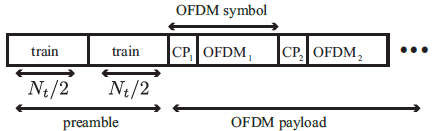
\includegraphics[scale=0.8]{img/operation_ofdm.png}
\caption{Representation of what's being done by the OFDM modulation}
\label{fig1}
\end{figure}

\section{Pre-lab}

In the first part of the lab, we have implemented an OFDM modulator  and the corresponding demodulator. First, at the transmitter side

\begin{itemize}

\item We have a sequence of $N-K$ symbols where N is the number of subcarriers and K is the number of null subcarrier.

\item \textbf{Null symbols} are inserted into groups of $N-K$ transmit suymbols.

\item We have an \textbf{IFFT} of the previous symbols.

\item Then, a \textbf{cyclic prefix} of length $L_c$ is added at the transmitter.

\end{itemize}

Second, at the receiver side

\begin{itemize}

\item The receiver consider block of $N+L_c$ without regarding the first $L_c$ samples of each block.

\item Then, we take back the \textbf{FFT} of the N symbols.

\end{itemize}

This previous 'operations' are represented on the block diagam on the figure \ref{fig2} and \ref{fig3}.

\begin{figure}[!ht]
    \begin{minipage}[b]{0.48\linewidth}
        \centering 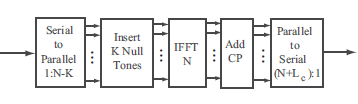
\includegraphics[scale=0.9]{img/OFDDM_modulator.png}
     \caption{Block diagram of the OFDM modulator}
     \label{fig2}
    \end{minipage}\hfill
    \begin{minipage}[b]{0.48\linewidth}
         \centering 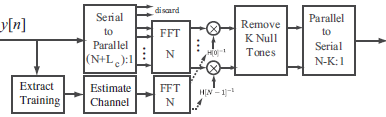
\includegraphics[scale=0.9]{img/OFDDM_demodulator.png}
 \caption{Block diagram of the OFDM demodulator}\label{fig3}
    \end{minipage}
\end{figure}


\section{Lab experiment}

\subsection{what is the respective OFDM symbol rate in the narrowband and wideband systems you have set up ?}

For $N=64$, and $L_c=8$

\begin{center}
	\begin{tabular}{c|c|c}
		  & Narrowband & Wideband\\
		  \hline
	Tx Sample rate & 4 $MSample/s$ & 20 $MSample/s$ \\	  
	Tx Oversample factor & 20 & 4\\
	\textbf{ODFM symbol rate} &  $\textbf{2777.77 symbol/s}$ & $\textbf{69444.44 symbol/s}$ \\ 
	\end{tabular}
	\label{tab1}
\end{center}

We simply have calculated the OFDM symbol rate by using the following formula

\begin{equation}
OFDM~symbol~rate = \frac{Tx~sample~rate}{N*L_c*Tx~oversample~factor}
\end{equation}

We can directly see that the symbol period is greater in a narrowband channel the in an wideband channel. (important for the future question). 

\subsection{What are the effective lengths of the narrowband and wideband channels respectively?}

If we take a look on the figure \ref{fig4} and \ref{fig5} representing the power delay in both case (narrow and wideband channel), we can deduce the effective length of the channel. The effective length is of $\textbf{2.5e-7~s}$ and $\textbf{1e-7~s}$ respectively for the narrowband and wideband channel.


\begin{figure}[!ht]
    \begin{minipage}[b]{0.48\linewidth}
        \centering 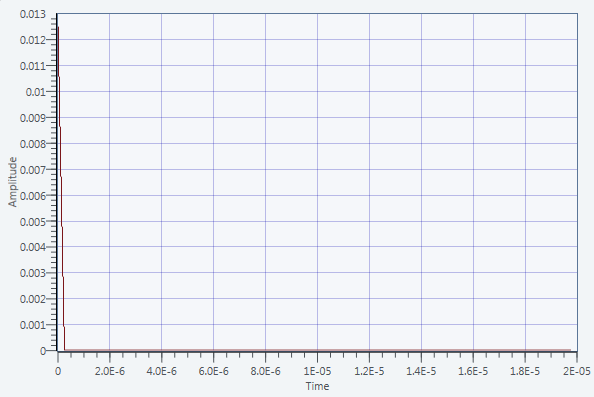
\includegraphics[scale=0.45]{img/power_delay_narrow.png}
     \caption{Power delay of the narrowband channel}
     \label{fig4}
    \end{minipage}\hfill
    \begin{minipage}[b]{0.48\linewidth}
         \centering 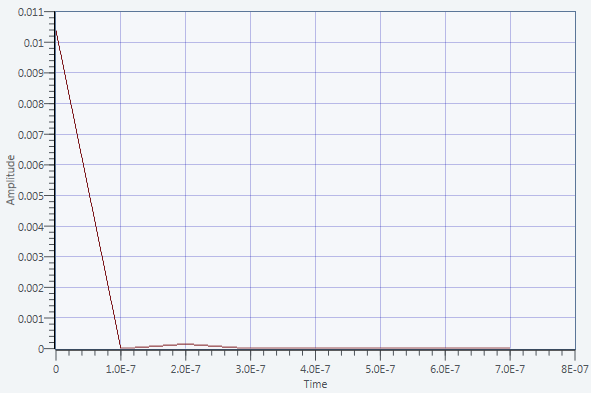
\includegraphics[scale=0.45]{img/power_delay_wideband.png}
 \caption{Power delay of the wideband channel}\label{fig5}
    \end{minipage}
\end{figure}


\subsection{Describe the frequency responses of each channel.}

\begin{figure}[!ht]
    \begin{minipage}[b]{0.48\linewidth}
        \centering 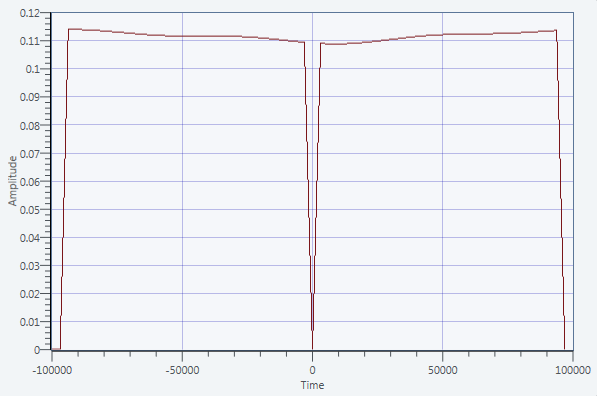
\includegraphics[scale=0.45]{img/channel_response_narrow.png}
     \caption{Response of a narrowband channel}
     \label{fig2}
    \end{minipage}\hfill
    \begin{minipage}[b]{0.48\linewidth}
         \centering 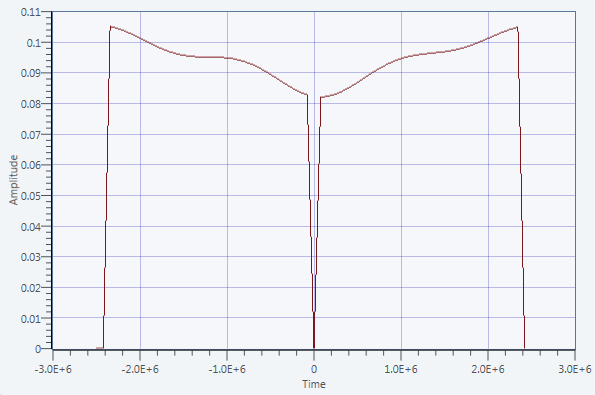
\includegraphics[scale=0.45]{img/channel_response_wideband.png}
 \caption{Response of a wideband channel}\label{fig3}
    \end{minipage}
\end{figure}


We can characterize a flat or a frequency-selective channel by comparing the bandwidth of the signal with the bandwidth of the channel (or the symbol period and the effective length).\\

\begin{itemize}
\item For a flat channel, we have that \textbf{Symbol period > Effective length of the channel}.
\item For a frequency-selective channel, we have just the inverse, \textbf{Symbol period < Effective length of the channel}.

\end{itemize}

By using the value computed in the previous question, we can deduce that

\begin{center}
	\begin{tabular}{c|c|c}
		  & Narrowband & Wideband\\
		  \hline
	Tx Sample rate & 4 $MSample/s$ & 20 $MSample/s$ \\	  
	Tx Oversample factor & 20 & 4\\
	\textbf{Symbol period} &  $\textbf{5e-6~s}$ & $\textbf{2e-7~s}$ \\ 
	\textbf{Delay spread}  &  $\textbf{2.5e-7~s}$ & $\textbf{1e-7~s}$ \\
	\end{tabular}
	\label{tab1}
\end{center} 












































\begin{comment}
\begin{figure}[!ht]
    \begin{minipage}[b]{0.48\linewidth}
        \centering 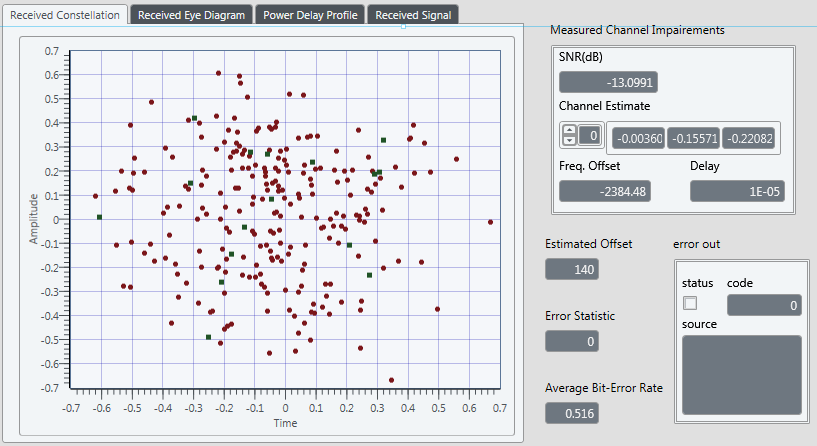
\includegraphics[scale=0.45]{img/Sliding_correletaion_OFF_AWGN_5dB_shift_bit_4.PNG}
     \caption{Error rate for a delay+4 in AWGN}
     \label{fig5}
    \end{minipage}\hfill
    \begin{minipage}[b]{0.48\linewidth}
         \centering 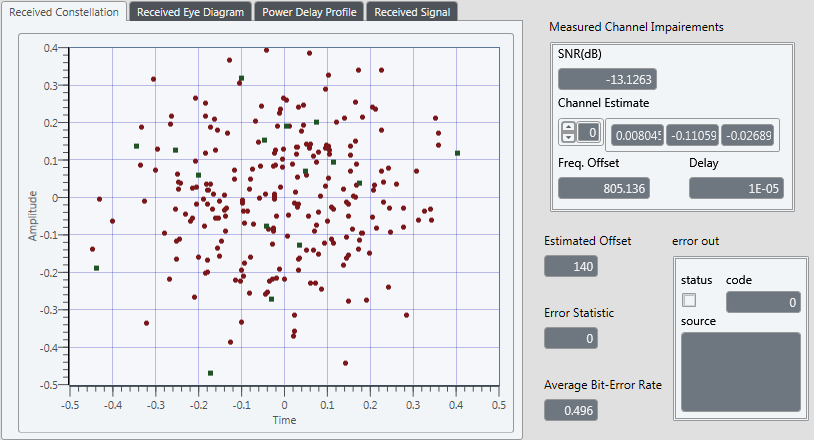
\includegraphics[scale=0.45]{img/Sliding_correletaion_OFF_AWGN_5dB_shift_bit_5.PNG}
 \caption{Error rate for a delay+5 in AWGN}\label{fig6}
    \end{minipage}
\end{figure}
\end{comment}


%\begin{figure}[!ht]
%\centering
%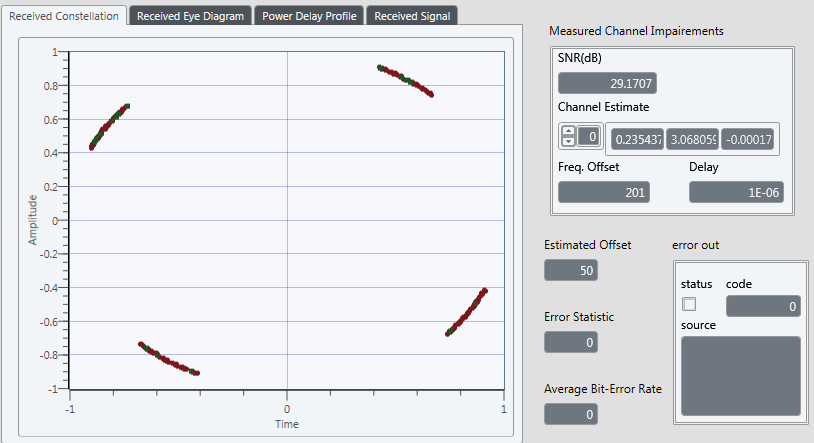
\includegraphics[scale=0.7]{img/test_offset_201hz_OFF.PNG}
%\caption{Constellation for a frequency offset of $201 \si{\hertz}$ without correction}
%\label{freq_correct_off}
%\end{figure}

%\begin{center}
%	\begin{tabular}{c|c}
%		Run & Frequency offset [\si{\hertz}]\\
%		\hline
%	\end{tabular}
%\end{center}


\end{document}
